
%\definecolor{Gcolor}{HTML}{3b528b}
%\definecolor{Dcolor}{HTML}{e41a1c}

%\definecolor{Gcolor}{HTML}{4477aa}
%\definecolor{pcolor}{HTML}{ee6677}
%\definecolor{dcolor}{HTML}{228833}

\definecolor{Gcolor}{HTML}{f03b20}
\definecolor{pcolor}{HTML}{0077bb}
\definecolor{dcolor}{HTML}{2c7fb8}

%\definecolor{Gcolor}{HTML}{004488}
%\definecolor{pcolor}{HTML}{bb5566}
%\definecolor{dcolor}{HTML}{ddaa33}

\tikzstyle{theory} = [thick, rectangle, rounded corners, minimum width=1.5cm, minimum height=1cm,text centered, draw=Gcolor]
\tikzstyle{nature} = [thick, rectangle, rounded corners, minimum width=1.5cm, minimum height=1cm,text centered, draw=pcolor]
\tikzstyle{none} = [thick, rectangle, rounded corners, minimum width=3.5cm, minimum height=1cm,text centered, draw=black]
\tikzstyle{io} = [thick,circle, trapezium left angle=70, trapezium right angle=110, minimum width=1.2cm, minimum height=1cm, text centered, draw=black]

\tikzstyle{cond} = [thick, rectangle, dotted, rounded corners, minimum width=4.2cm, minimum height=7cm,text centered, draw=gray!50!black]

\tikzstyle{iodotted} = [thick, circle, trapezium left angle=70, trapezium right angle=110, minimum width=1.2cm, minimum height=1cm, text centered, draw=black, dotted]

\tikzstyle{process} = [thick, rectangle, minimum width=1cm, minimum height=1cm, text centered, draw=black]

\tikzstyle{xG} = [thick,rectangle, minimum width=2.2cm, minimum height=3cm, text depth= 2.2cm, draw=black]
\tikzstyle{s0} = [thick,rectangle, minimum width=2cm, minimum height=3cm, text centered]
\tikzstyle{s1} = [thick, dotted, rectangle, minimum width=1.6cm, minimum height=1.1cm, text centered, draw=black]


\tikzstyle{decision} = [thick,rectangle, minimum width=1cm, minimum height=1cm, text centered, draw=black]


\tikzstyle{dots} = [circle, minimum size=2pt, inner sep=0pt,outer sep=0pt, draw=Dcolor, fill = Dcolor]

\tikzstyle{arrow} = [thick,->,>=stealth]

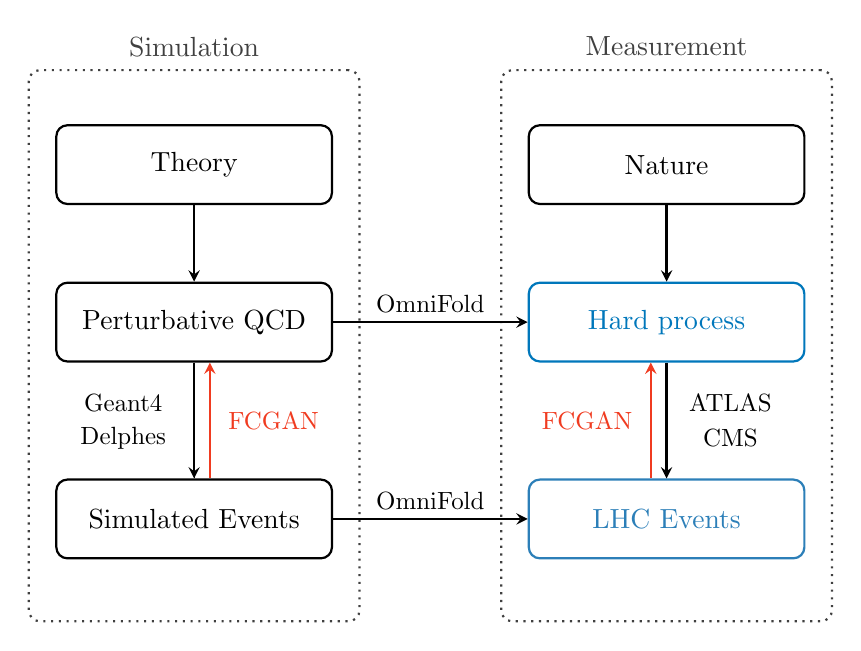
\begin{tikzpicture}[node distance=2cm]


\node (theory) [none] {Theory};
\node (nature) [none, right of = theory, xshift = 4cm] {Nature};

\node (parton) [none, below of = theory, color = black] {Perturbative QCD};
\node (hard) [none, color = pcolor, below of = nature] {Hard process};

\node (mcevent) [none, below of = parton, yshift=-0.5cm, color = black] {Simulated Events};
\node (data) [none, color = dcolor, below of = hard, yshift=-0.5cm] {LHC Events};


\node (theorybig)[cond, below of = theory, yshift=-0.3cm]{};
\node (theorybig)[cond, below of = nature, yshift=-0.3cm]{};
\node(theo1)[above of = theory, color=gray!50!black,yshift=-0.5cm]{Simulation};
\node(theo1)[above of = nature, color=gray!50!black,yshift=-0.5cm]{Measurement};

\draw[arrow] (theory) -- (parton);
\draw[arrow] (nature) -- (hard);
\draw[arrow] (parton) --  node[scale=0.9, below, anchor=center, xshift=-1.0cm, yshift=0.25cm] {Geant4} (mcevent);
\draw (parton) -- node[scale=0.9, below, anchor=center, xshift=-1.0cm, yshift=-0.25cm] {Delphes} (mcevent);

\draw[arrow] (hard) --node[scale=0.9, above, anchor=center, xshift=0.9cm, yshift=0.25cm] {ATLAS}  (data);
\draw (hard) --node[scale=0.9, above, anchor=center, xshift=0.9cm, yshift=-0.25cm] {CMS}  (data);

\draw[arrow] (parton) -- node [scale=0.9, above] {OmniFold} (hard);
\draw[arrow] (mcevent) -- node [scale=0.9, above] {OmniFold}  (data);

\draw[arrow, color=Gcolor] ([xshift=0.2cm] mcevent.north) -- node [scale=0.9,below, anchor=center, xshift=0.9cm ] {FCGAN} ([xshift=0.2cm]parton.south);
\draw[arrow, color=Gcolor] ([xshift=-0.2cm] data.north) -- node [scale=0.9,above,anchor=center, xshift=-0.9cm ] {FCGAN} ([xshift=-0.2cm]hard.south);








\end{tikzpicture}
